\section{相位框架与局部几何}
\label{core:framework}

为了在保持测量正交性的同时调节局部几何，将可调参数放入对角相位。对$n\ge2$，采用计算基$\ket{z_1\cdots z_n}$，其中$z_j\in\mathbb F_2$，门序沿用文献~\cite{PauwelsGisin2026}，矩阵乘积从右向左作用。记
\begin{align}
 C_n&=S(n)H_n,\qquad M[D]=C_nDH^{\otimes n},\nonumber\\
 S(n)&=\mathrm{CNOT}_{2\to1}\cdots\mathrm{CNOT}_{n\to n-1},
 \label{core:phase-family}
\end{align}
其中$H_n$只作用于末位比特，$D$为各对角元模长均为一的对角矩阵。由酉性，对每个这样的$D$，全部列$\ket{\psi_k}=M[D]\ket{k}$都构成正交完备测量。各列的局部几何由种子态$\ket{\psi_0}$决定：将列标签写为$k=(e_1,\ldots,e_{n-1},\sigma)$，其中$e\in\mathbb F_2^{n-1}$、$\sigma\in\mathbb F_2$，则有精确的Pauli轨道恒等式
\begin{equation}
 \ket{\psi_{e,\sigma}}=
 \left[\prod_{h=1}^{n-1}(Z_hZ_{h+1})^{e_h}\right]
 (X^{\otimes n})^\sigma\ket{\psi_0}.
 \label{core:orbit}
\end{equation}
这一轨道将种子的局部Bloch向量传递到全部测量列。要得到共同半径的正四面体，只需使种子的带符号局部分量相等。全文固定局部坐标：仅对末位比特的$Y$分量作符号调整，$\widetilde Y_n=-Y_n$；其余$\widetilde P$均等于相应的物理Pauli算符。因此，共同带符号分量$m\ge0$对应的种子Bloch向量为：$j<n$时$m(1,1,1)$，$j=n$时$m(1,-1,1)$。

相位变形从指定基点出发，其相位为
\begin{equation}
 \begin{aligned}
 f_0(z)&=\sum_{\ell=2}^n(-1)^\ell e_\ell(z)\\
 &=\begin{cases}0,&z=0,\\ |z|-1,&z\ne0,\end{cases}\pmod4.
 \end{aligned}
 \label{core:reference-phase}
\end{equation}
其中$e_\ell$为基本对称多项式，$|z|$为Hamming重量。基点测量取$D_0(z)=i^{f_0(z)}$，其半径为
\begin{equation}
 c_n=2^{1-n},\qquad r_E(n)=\sqrt3\,c_n.
 \label{core:reference-radius}
\end{equation}

为计算种子的带符号分量，将种子态分解为背景态与物理全零串处的单点修正。对$\mathbb F_2^n$上任意实函数$\Theta$，定义
\begin{align}
 \ket{\chi_\Theta}&=2^{-n/2}\sum_z i^{|z|}e^{i\Theta(z)}\ket z,\nonumber\\
 D_\Theta(z)&=\begin{cases}1,&z=0,\\
 i^{f_0(z)}e^{i\Theta(z)},&z\ne0.
 \end{cases}
 \label{core:background}
\end{align}
种子态严格满足
\begin{equation}
 \ket{\psi_0}=-iC_n\left[\ket{\chi_\Theta}
 +2^{-n/2}\big(i-e^{i\Theta(0)}\big)\ket{0^n}\right].
 \label{core:defect-state}
\end{equation}
无论如何表示$\Theta$，该修正只改变一个物理输入的振幅。

\begin{lemma}[局部相位机制]
\label{core:mechanism}
对带符号的局部Pauli算符，记
\begin{equation}
 R=C_n^\dagger\widetilde P C_n=i^kX^aZ^b,\quad
 h=a\oplus b,\quad\Gamma=i^{k-|a|},
 \label{core:pauli-notation}
\end{equation}
并令$B_R=\bra{\chi_\Theta}R\ket{\chi_\Theta}$，则
\begin{equation}
 \langle\widetilde P\rangle
 =B_R+c_n\operatorname{Re}\!\left[
 \Gamma e^{-i\Theta(a)}\big(i-e^{i\Theta(0)}\big)\right].
 \label{core:signal}
\end{equation}
若所有带符号期望均等于$m\ge0$，则每个测量列的真实单比特约化态为
\begin{equation}
 \rho_{j,e,\sigma}
 =\frac12\left[I+\sqrt3m\,\mathbf v_{j,\kappa_j,\sigma}
 \cdot\boldsymbol\sigma\right],
 \label{core:bloch-orbit}
\end{equation}
其中$e_0=e_n=0$、$\kappa_j=e_{j-1}\oplus e_j$，且
\begin{equation}
 \begin{aligned}
 \mathbf v_{j,q,s}&=\frac1{\sqrt3}
 \big((-1)^q,\epsilon_j(-1)^{q+s},(-1)^s\big),\\
 \epsilon_j&=\begin{cases}1,&j<n,\\-1,&j=n.\end{cases}
 \end{aligned}
 \label{core:vertices}
\end{equation}
对每个$j$，这四个单位向量构成正四面体，每个标签$(q,s)$恰出现$2^{n-2}$次。
\end{lemma}

所有拉回算符均满足$a\ne0$，所以式\eqref{core:defect-state}中的修正对局部期望没有对角贡献；两个交叉项给出式\eqref{core:signal}。由式\eqref{core:orbit}中的轨道算符作共轭，即得式\eqref{core:vertices}的四面体符号。附录\ref{core:appendix}给出逐门拉回及约化态推导。

对Boolean相位$\Theta=tq$且$q(0)=1$，拉回算符分为两类：I类满足$\Gamma=-i$、$h\cdot a=1$；II类满足$\Gamma=-1$、$h\cdot a=0$。定义归一化Walsh系数
\begin{equation}
 \begin{aligned}
 W_q(h)&=2^{-n}\sum_z(-1)^{q(z)\oplus h\cdot z},\\
 D_aq(z)&=q(z)\oplus q(z\oplus a).
 \end{aligned}
 \label{core:walsh-def}
\end{equation}
则背景项为
\begin{equation}
 B_R(t)=\begin{cases}
 -\sin t\,W_q(h),&\text{I类},\\
 -\sin^2(t/2)\,W_{D_aq}(h),&\text{II类}.
 \end{cases}
 \label{core:boolean-background}
\end{equation}
这些公式将背景项写成相位函数及其导数的Walsh系数。

\section{全部\texorpdfstring{$n\ge5$}{n >= 5}的统一族}
\label{core:unified}

式\eqref{core:signal}给出两项设计要求：消去所有背景项$B_R(t)$，并使剩余交叉项相等。对Boolean相位，前者化为式\eqref{core:boolean-background}中的Walsh消去条件，后者确定局部翻转处的取值$q(a)$。对每个整数$n\ge5$，四个线性特征将这两项要求归约为同一个四位核上的条件。定义两个内部奇偶块
\begin{equation}
 \begin{aligned}
 E_n&=\{2,4,\ldots\}\cap[2,n-2],\\
 O_n&=\{3,5,\ldots\}\cap[2,n-2],
 \end{aligned}
\end{equation}
以及四个线性特征
\begin{align}
 x&=z_1\oplus z_{n-1},& b&=\bigoplus_{j\in E_n}z_j,\nonumber\\
 c&=\bigoplus_{j\in O_n}z_j,& s&=z_1\oplus z_n.
 \label{core:features}
\end{align}
记$\mathcal L_nz=(x,b,c,s)$。两个内部块均非空，四个特征线性无关。在$\mathbb F_2^4$上取
\begin{equation}
 F(x,b,c,s)=\begin{cases}
 1\oplus(1\oplus c)(x\oplus b),&s=0,\\
 b\oplus xc,&s=1.
 \end{cases}
 \label{core:kernel}
\end{equation}
令
\begin{equation}
 q_n(z)=F(\mathcal L_nz),\qquad
 d_n(z)=q_n(z)-\delta_{z,0}.
 \label{core:support}
\end{equation}
这里的减法取整数意义。因为$F(0)=1$，$d_n$仍为Boolean函数。被移除的只有物理全零串，不是整个纤维$\mathcal L_nz=0$。

图~\ref{fig:unified}(a)展示同一四特征核如何确定每个$n\ge5$的相位；图(b)给出以$r_E(n)$归一化的半径变化。
\begin{figure*}[tbp]
  \centering
  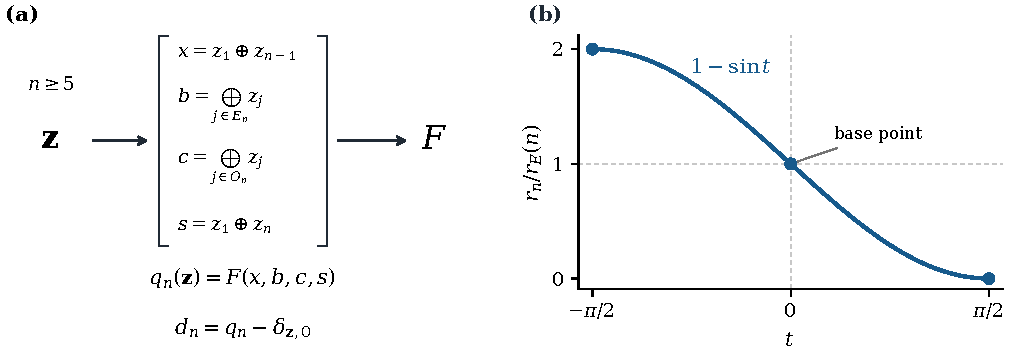
\includegraphics[width=\textwidth]{figures/fig1_unified.pdf}
  \caption{Unified phase deformation for every $n\geq5$.
  (a) Four linear Boolean features feed the same kernel $F$; the only removed support point is the physical string $\mathbf z=0$.
  The blocks $E_n$ and $O_n$ contain the even and odd indices in $[2,n-2]$, respectively.
  (b) The normalized common Bloch radius $r_n(t)/r_E(n)=1-\sin t$ on $[-\pi/2,\pi/2]$, where $r_E(n)=\sqrt3/2^{n-1}$ is the reference radius.
  From left to right, the marked points give the enhanced endpoint, the specified EJM at $t=0$, and the endpoint with maximally mixed one-qubit marginals.}
  \label{fig:unified}
\end{figure*}

\begin{theorem}[统一增强族]
\label{core:unified-theorem}
对每个整数$n\ge5$，令
\begin{equation}
 D_{n,t}(z)=i^{f_0(z)}e^{itd_n(z)},\qquad
 M_n(t)=C_nD_{n,t}H^{\otimes n}.
 \label{core:unified-measurement}
\end{equation}
对每个实数$t$，全部列均构成正交归一基，其单比特约化态由式\eqref{core:bloch-orbit}给出，其中
\begin{equation}
 m_n(t)=c_n(1-\sin t),\qquad
 r_n(t)=r_E(n)(1-\sin t).
 \label{core:radius}
\end{equation}
四面体方向与$t$无关。在区间
\begin{equation}
 J=[-\pi/2,\pi/2],\qquad r_n(J)=[0,2r_E(n)],
 \label{core:interval}
\end{equation}
半径连续且严格递减。$t=0$逐列恢复基点测量；$t=-\pi/2$达到半径$2r_E(n)$；$t=\pi/2$时全部单比特约化态均为$I/2$。
\end{theorem}

\begin{proof}
证明将随维数变化的特征映射与六个固定的四位消去恒等式分开。首先，形如
\begin{equation}
 2^{-n}\sum_z(-1)^{h\cdot z}G(\mathcal L_nz)
 \label{core:pairing-sum}
\end{equation}
的和式，在$h$不属于$\mathcal L_n$行空间时为零：取$\mathcal L_nw=0$、$h\cdot w=1$的平移$z\mapsto z\oplus w$，每一项的符号均反转。当$h$属于行空间时，写成$h=\mathcal L_n^TH$，利用各纤维等大，将式\eqref{core:pairing-sum}化为$2^{-4}\sum_v(-1)^{H\cdot v}G(v)$。对$q_n$的导数同样适用，因为$D_aq_n=(D_AF)\circ\mathcal L_n$，其中$A=\mathcal L_na$。

其次，逐门拉回表中的局部字符只留下以下条件：
\begin{align}
 W_F(9)&=W_F(11)=W_F(15)=0,\nonumber\\
 W_{D_6F}(6)&=W_{D_7F}(13)=W_{D_7F}(11)=0.
 \label{core:six-cancellations}
\end{align}
整数按$(x,b,c,s)$编码，$x$为最高位；Walsh系数的归一化因子为$2^{-4}$。六个和式均可通过特征位配对消去。附录~\ref{core:alln-classification}给出有限计算，并证明这六式覆盖每个$n\ge5$的全部局部分量，包括$n=5,6,7$的额外残留项。由式\eqref{core:boolean-background}，$B_R(t)$恒为零。

最后，所有I类翻转均满足$F(\mathcal L_na)=0$，所有II类翻转均满足$F(\mathcal L_na)=1$。式\eqref{core:signal}分别化为
\begin{align}
 c_n\operatorname{Re}[-i(i-e^{it})]&=c_n(1-\sin t),\nonumber\\
 c_n\operatorname{Re}[-e^{-it}(i-e^{it})]&=c_n(1-\sin t).
\end{align}
引理\ref{core:mechanism}把种子恒等式传递到全部测量列。端点、基点与精确像的结论由对角相位以及$\sin t$在$J$上的严格单调性得到。
\end{proof}

该增强具有直接的单比特纠缠含义。所有测量结果、所有$1|(n-1)$划分共享同一局部谱
\begin{equation}
 \lambda_\pm=\frac{1\pm r_n(t)}2,
 \qquad \operatorname{Tr}\rho_j^2=\frac{1+r_n(t)^2}{2}.
 \label{core:spectrum}
\end{equation}
相应的熵为$h_2((1+r_n(t))/2)$，其中$h_2(p)=-p\log_2p-(1-p)\log_2(1-p)$，端点值按连续性定义。Bloch半径增加时，这一二分纠缠下降。$t=\pi/2$时，式\eqref{core:defect-state}的单点修正消失；$t=-\pi/2$时，其干涉产生基点两倍的局部信号。四个线性特征足以表示全部$n$的相位，但提取这些特征仍依赖物理寄存器的大小。



